\documentclass{article}

% Language setting
% Replace `english' with e.g. `spanish' to change the document language
\usepackage[english]{babel}

% Set page size and margins
% Replace `letterpaper' with `a4paper' for UK/EU standard size
\usepackage[letterpaper,top=2cm,bottom=2cm,left=3cm,right=3cm,marginparwidth=1.75cm]{geometry}

% Useful packages
\usepackage{amsmath}
\usepackage{graphicx}
\usepackage[colorlinks=true, allcolors=blue]{hyperref}
\usepackage{wrapfig}

\title{\textbf{Deflection of Electrons in Presence of Electric and Magnetic Field}}
\author{Riddhiman Bhattacharya}



\begin{document}
\maketitle



\section{\Large Introduction}
\large

Here we'll try to inquire about the behavior of electrons when exposed to magnetic fields.

\section{\Large Mathematical Calculations and Theories}
\large


Let's consider a beam of particles with charge $q$ mass $m$ moving at velocity $v$ through vaccum. If there is a presence of a uniform electric field $\vec{E}
$ and uniform magnetic field $\vec{B}
$, the force on each particle is given by Lorentz Force 

$$ \vec{F}=q\vec{E}+ q\vec{v} \times \vec{B} $$

\subsection{\Large Diagram}
\large

Before moving to the actual calculation, let us see the arrangement for the magnetic deflection of the charged particles.

\begin{figure}
\centering
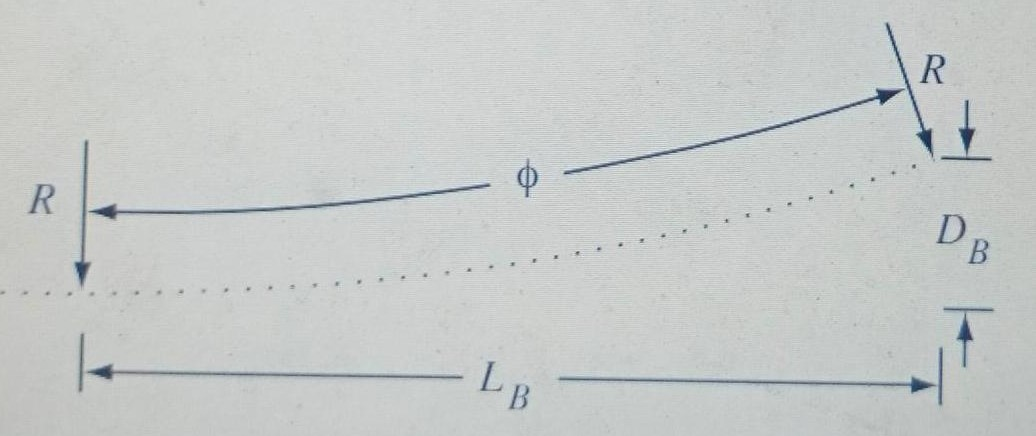
\includegraphics[width=0.5\linewidth]{Deflection of Electrons.jpeg}
\caption{Arrangements for Magnetic Deflection of Charged Particles. Magnetic field is distributed uniforly over the entire distance $L_B$}

\end{figure}
\subsection{\Large Derivation}
\large 
The magnetic force is constant and perpendicular to $\vec{u}$. The particles will
move in a circular trajectory and it's radius can be found out by equating the magnetic force to the centripetal
force needed to move in a circle of radius $R$.

$$qvB=\frac{{mv^2}}{{R}}$$

 $$R = \frac{{mv}}{{qb}}$$

 The total deflection $D_B$ can be written from the figure as

 $$ D_B= R - R \cos(\phi)$$

 Because the angle is very small, we'll use small angle approximations to get our final results

 $L_B\approx R\phi$ and $\cos(\phi)\approx 1-\frac{{\phi^2}}{{2}}
$

Substituting the values in total deflection $D_B$, we get 

$$D_B=\left(\frac{{q}}{{m}}\right) \left(\frac{{(L_B)^2}}{{2v}}\right) B
$$










\end{document}